\chapter{Methodology}
\label{chap:2}
\ChapterPageStuff{2}

\section{Preamble} The literature in \Cref{chap:1} is used for the method to create a logging mechanism that can capture user-based activity logs to improve software maintenance by analysing the obtained logs.\par In \Cref{Ch2:LoggingMechanism} the methodology to create a logging mechanism to capture user-generated events is discussed for web-based applications. The different functional requirements and interfaces are discussed in this section \cite{Anish2015}.\par In \Cref{ch2:system_utilisation_analysis} the methodology is discussed to analyse these obtained logs to improve software maintenance.

\section{Logging mechanism}\label{Ch2:LoggingMechanism} The logging mechanism will need to meet the requirements discussed in \Cref{sec:EventLogging} to capture the required logs to apply system utilisation analysis on it. \Cref{fig:CH2_SystemA_Arch_Design} is the design for the logging mechanism to capture the user's activities. In this figure, the logging mechanism is split up into two functional requirements parts (F/R) which consist of the client and server functional requirements.\par Each functional requirement has an interface requirement that transfers the data from one interface to another interface. These interfaces are labeled as I/F in \Cref{fig:CH2_SystemA_Arch_Design}. The \Cref{fig:CH2_SystemA_Arch_Design} is the client interface (F/R 1) and the server interface (F/R 2) that forms the entire logging mechanism to capture the user-based activity logs.

\begin{figure}[!htb] % An h :here, t: top, b: bottom.
	\centering % cent the figure
	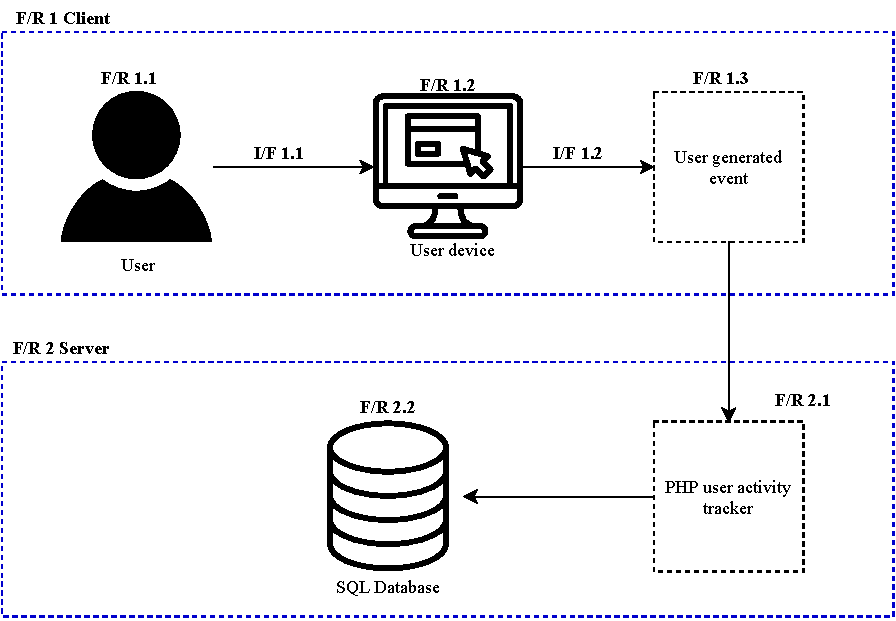
\includegraphics[width=0.9\textwidth]{Chapter2/SystemA_Architecture_Diagram/SystemA_Architecture_Diagram.pdf}
	\caption[System A logging mechanism architecture design]
	{\textit{System A logging mechanism architecture design}}\label{fig:CH2_SystemA_Arch_Design}
\end{figure}

\clearpage

\subsection{Clients functional requirements}

The client's functional requirements (F/R 1) are where the user-based activity is triggered. In \Cref{fig:ch2_SystemA_Arch_Design} the client interface consists of the of three main parts that include the:

\begin{itemize}
	\item The user (F/R 1.1),
	\item The user's device (F/R 1.2) which they access the software
	\item The user-generated event log (F/R 1.3).
\end{itemize}

In \Cref{tbl:Ch2_Client_Functional_Requirements} is the functional requirements describe above in m that are on the client-side of the user activity logging mechanism.

\begin{table}[!htb]
	\centering
	\small
	\caption[Client functional requirements]
	{\textit{Client functional requirements (F/R 1)}}
	\label{tbl:Ch2_Client_Functional_Requirements}
	\begin{tabularx}{\textwidth}{|l|l|X|}
		\hline \textbf{Requirement ID} & \textbf{Name} & \textbf{Description} \\
		\hline F/R 1.1 & User & The user serves as the primary initiator of the activity events.\\
		\hline F/R 1.2 & User's device & The device that the user uses to access the website from where the activity events are generated.\\
		\hline F/R 1.3 & User-generated events & These are any activity events that the user started that need to communicate back to the server.\\
		\hline
	\end{tabularx}
\end{table}

\subsubsection{Requirements for an event log to be classified as a user-based activity}
The user is the initiator of the logging mechanism. Each action or event they trigger by interacting with the user interface on their device (F/R 1.2) can be a potential user-generated event. In \Cref{tbl:ch2_requirementsForUserActivtyEvent} is the sub-requirements for the user (F/R 1.1) which the event log should fulfill to be classified as an user-based activity log.

\begin{table}[!htb]
	\centering
	\small
	\caption[Requirements for an event to be a user-based activty]
	{\textit{Requirements for an event to be a user-based activty}}
	\label{tbl:ch2_requirementsForUserActivtyEvent}
	\begin{tabularx}{\textwidth}{|l|X|}
		\hline \textbf{Requirement ID} & \textbf{Description}\\
		\hline F/R 1.1.1 & The event has to be triggered by the user interacting with the user interface. \\
		\hline F/R 1.1.2 & The event must consists of different cases ($ca~ \epsilon~CA$ the cases consists of events) which are noteworthy to make the event log identifiable \cite{Slaninova2014}. \\
		\hline F/R 1.1.3 & The event log should consist of attributes. \\
		\hline
	\end{tabularx}
\end{table}

Every interaction the user has with the user interface of the device to the software system can be seen as an event triggered by the user. Most of these events won't have meaningful impact as they won't fulfill F/R 1.1.2 and F/R 1.1.3 in \Cref{tbl:ch2_requirementsForUserActivtyEvent}.\par For the user activity event to meet the requirement of 1.1.2 it has to have defined cases that describe the activity type of each event. These activity types form the basic criteria for which event can be parsed which significantly reduces the number of logs that will be obtained. This will ensure that the event logging process will produce quality user-based logs as discussed in \Cref{sec:CH1_LoggingQuality}:

\begin{itemize}
	\item A basic structural complexity to simplify log parsing,
	\item Increase accuracy by only obtaining the logs that are part of the different defined cases,
	\item Keep the logging consistent by not deviating from the defined cases, and
	\item Ensure that the event log's other attributes are complete and available
\end{itemize}

\clearpage

As previously stated this logging mechanism is for web-based applications, therefore the user activity types need to be established for these types of applications. Web applications consist of different page architectures. The Model-View-Controller (MVC) architecture is mostly used for web-based applications.\par The MVC architecture in \Cref{fig:ch2_flowMVC_Architecture} consists of 3 basic parts which are the \cite{Jailia2016}:

\begin{itemize}
	\item \textit{Model:} Is the representation of the records in the database which also interacts with the database through a database access layer or service.
	\item \textit{Controller:} Is operates both the \textit{View} and \textit{Model} and serves as the connection between the user and the system by controlling the data flow of the \textit{Model} and \textit{View}.
	\item \textit{View:} This shows the results of the data contained in the \textit{Model} and enables the user to manipulate the data.
\end{itemize}

\begin{figure}[!htb] % An h :here, t: top, b: bottom.
	\centering % cent the figure
	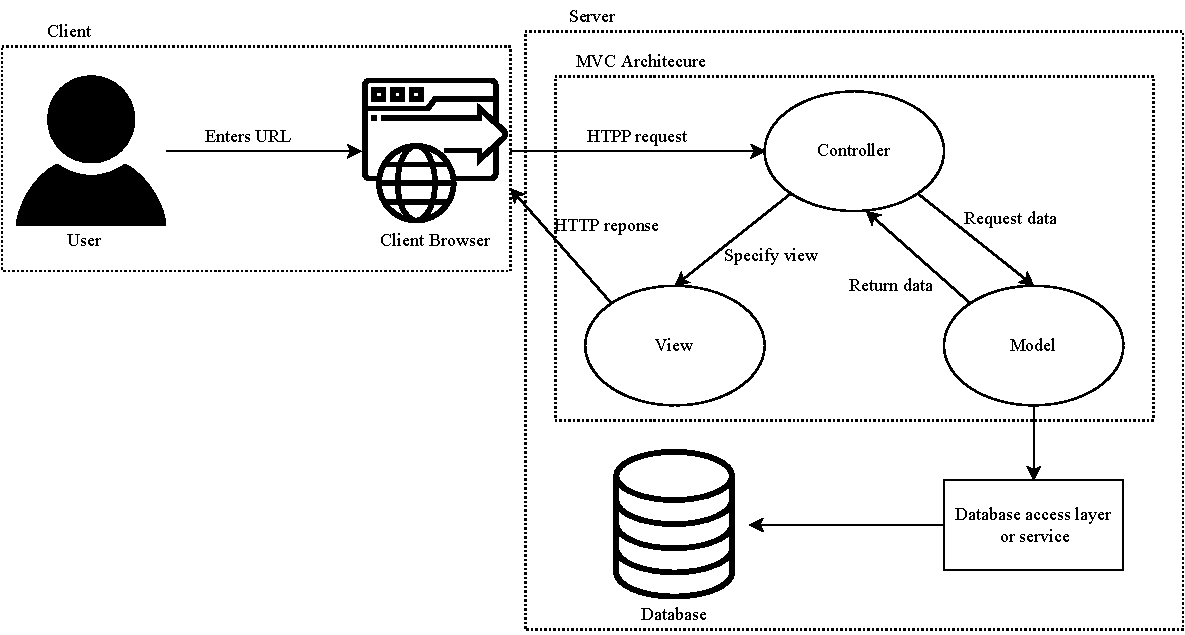
\includegraphics[width=0.85\textwidth]{Chapter2/Flow_MVC_Architecture/Flow_MVC_Architecture.pdf}
	\caption[Request flow in MVC architecture]
	{\textit{Request flow in MVC architecture \cite{Gu2010}}}\label{fig:ch2_flowMVC_Architecture}
\end{figure}

This flow of data in \Cref{fig:ch2_flowMVC_Architecture} depicts that any \textit{update}, \textit{create} and \textit{delete} event will have a request and response. Only the request can be used as that will possibly be an action that the user triggered.

\begin{table}[!htb]
	\centering
	\small
	\caption[User activity types]
	{\textit{User activity types}}
	\label{tbl:Ch2_User_ActivityTypes}
	\begin{tabularx}{\textwidth}{|l|X|}
		\hline \textbf{Activity Type} & \textbf{Description} \\
		\hline Page accessed & The user may enter different web pages in a session. Tracking which pages the user navigates through.\\
		\hline Session changes & This is any user activities that directly involve an extension session before their session times out after a period of inactivity. This also tracks when the session starts as any login attempt is a user-based activity.\\
		\hline General user events & Any events that are other than accessing a certain web page that user initiates that communicates with the server. Most of the user activities will have this event type.\\ 
		\hline
	\end{tabularx}
\end{table}


\clearpage

The functional requirements in \Cref{tbl:Ch2_Client_Functional_Requirements} needs to interface with each other. These interfaces in \Cref{tbl:Ch2_Client_Interface_Requirements} parses the input from the user to create a basic user event log. 

\begin{table}[!htb]
	\centering
	\small
	\caption[Client interface requirements]
	{\textit{Client interface requirements for F/R 1}}
	\label{tbl:Ch2_Client_Interface_Requirements}
	\begin{tabularx}{\textwidth}{|l|l|X|}
		\hline \textbf{Requirement ID} & \textbf{Name} & \textbf{Description} \\
		\hline I/F 1.1 & User input & The user starts the activity events by using the user interface to give the website any input.\\
		\hline I/F 1.2 & Log parsing of logging points & The user-generated event is captured to get some of the key logging points of \Cref{tbl:CH1_Log_Basic_Attributes}.\\
		\hline
	\end{tabularx}
\end{table}

The server functional requirements in \Cref{tbl:Ch2_Server_Functional_Requirements} captures the rest of the key-logging points and complete the event log to be stored in a database. 

\begin{table}[!htb]
	\centering
	\small
	\caption[Server functional requirements]
	{\textit{Server functional requirements (F/R 2)}}
	\label{tbl:Ch2_Server_Functional_Requirements}
	\begin{tabularx}{\textwidth}{|l|l|X|}
		\hline \textbf{Requirement ID} & \textbf{Name} & \textbf{Description} \\
		\hline F/R 2.1 & User activity logger & The rest of the key logging points are captured and the event log is completed to stored in a database.\\
		\hline F/R 2.2 & Database & The event log is stored in a database until it is needed for further analysis.\\
		\hline
	\end{tabularx}
\end{table}

The interfaces in \Cref{tbl:Ch2_Server_Interface_Requirements} for the client functional requirement (F/R 2) is to obtain the base log from the client functional requirement (F/R 1) and finally store the completed log into a database.

\begin{table}[!htb]
	\centering
	\small
	\caption[Server interface requirements]
	{\textit{Server interface requirements for F/R 2}}
	\label{tbl:Ch2_Server_Interface_Requirements}
	\begin{tabularx}{\textwidth}{|l|l|X|}
		\hline \textbf{Requirement ID} & \textbf{Name} & \textbf{Description} \\
		\hline I/F 2.1 & Log parsing to server & The captured log is parsed onto the server for further processing of the captured user-generated event.\\
		\hline I/F 2.2 & Store in database & The event log is sent to a database for storing.\\
		\hline
	\end{tabularx}
\end{table}

\clearpage

\subsection{Logging points}
The required logging points should be defined to create the base event log. Before these logging points can be defined the logging attributes need to be defined as discussed in \Cref{sec:Ch1_LoggignPoints}. The defined logging attributes in \Cref{tbl:Ch2_KeyLogging_Attributes} are the base attributes that form the main structure of the event log. 

\begin{table}[!htb]
	\centering
	\small
	\caption[Key logging attributes]
	{\textit{Key logging attributes}}
	\label{tbl:Ch2_KeyLogging_Attributes}
	\begin{tabularx}{\textwidth}{|l|X|}
		\hline \textbf{Logging point} & \textbf{Description} \\
		\hline Identification number & The activity identification is an incremental number of the event that is logged.\\
		\hline Timestamp & This is the time which the event took place.\\
		\hline Activity type & Each event can be classified into types. This is the user activity types in \Cref{tbl:Ch2_User_ActivityTypes} \\
		\hline User identification & Each user has a unique identification number that links the event to them. \\
		\hline Request origin & In web applications, there are always requests sent back to the server and will call the primary function to handle the request. The file in which the function is the request origin. \\
		\hline Metadata & The metadata of the event contains request parameters, the HTML element from which the request is initiated and other relevant request data of the event. This can also be other metadata important to get that adds more information about the user's activity. In \Cref{fig:Ch2_Metadata_Json_Example} is an example representation of the metadata. \\
		\hline
	\end{tabularx}
\end{table}

Each logging point 



\begin{figure}[!htb]
	\centering
	\begin{lstlisting}[style=json] 
		{ "RequestOrigin" : "/Area4/Controller4",
		  "RequestElementID" : "Button4",
		  "RequestParameters": {
		  "Parameter1": 4,
		  "Parameter2": "Hello World!",
			"Parameter3": true
			"Parameter4": 40.404
		  }		
		}
	\end{lstlisting}
	\caption[System B metadata JSON]
	{\textit{System B metadata JSON}}\label{fig:Ch2_Metadata_Json_Example}
\end{figure}

\section{System utilisation analysis}\label{ch2:system_utilisation_analysis}

\section{integration}

\section{Conclusion}